\chapter{PK10 --- Tác vụ định kỳ}
\clearpage\begin{landscape}
\begin{figure}[H]\centering
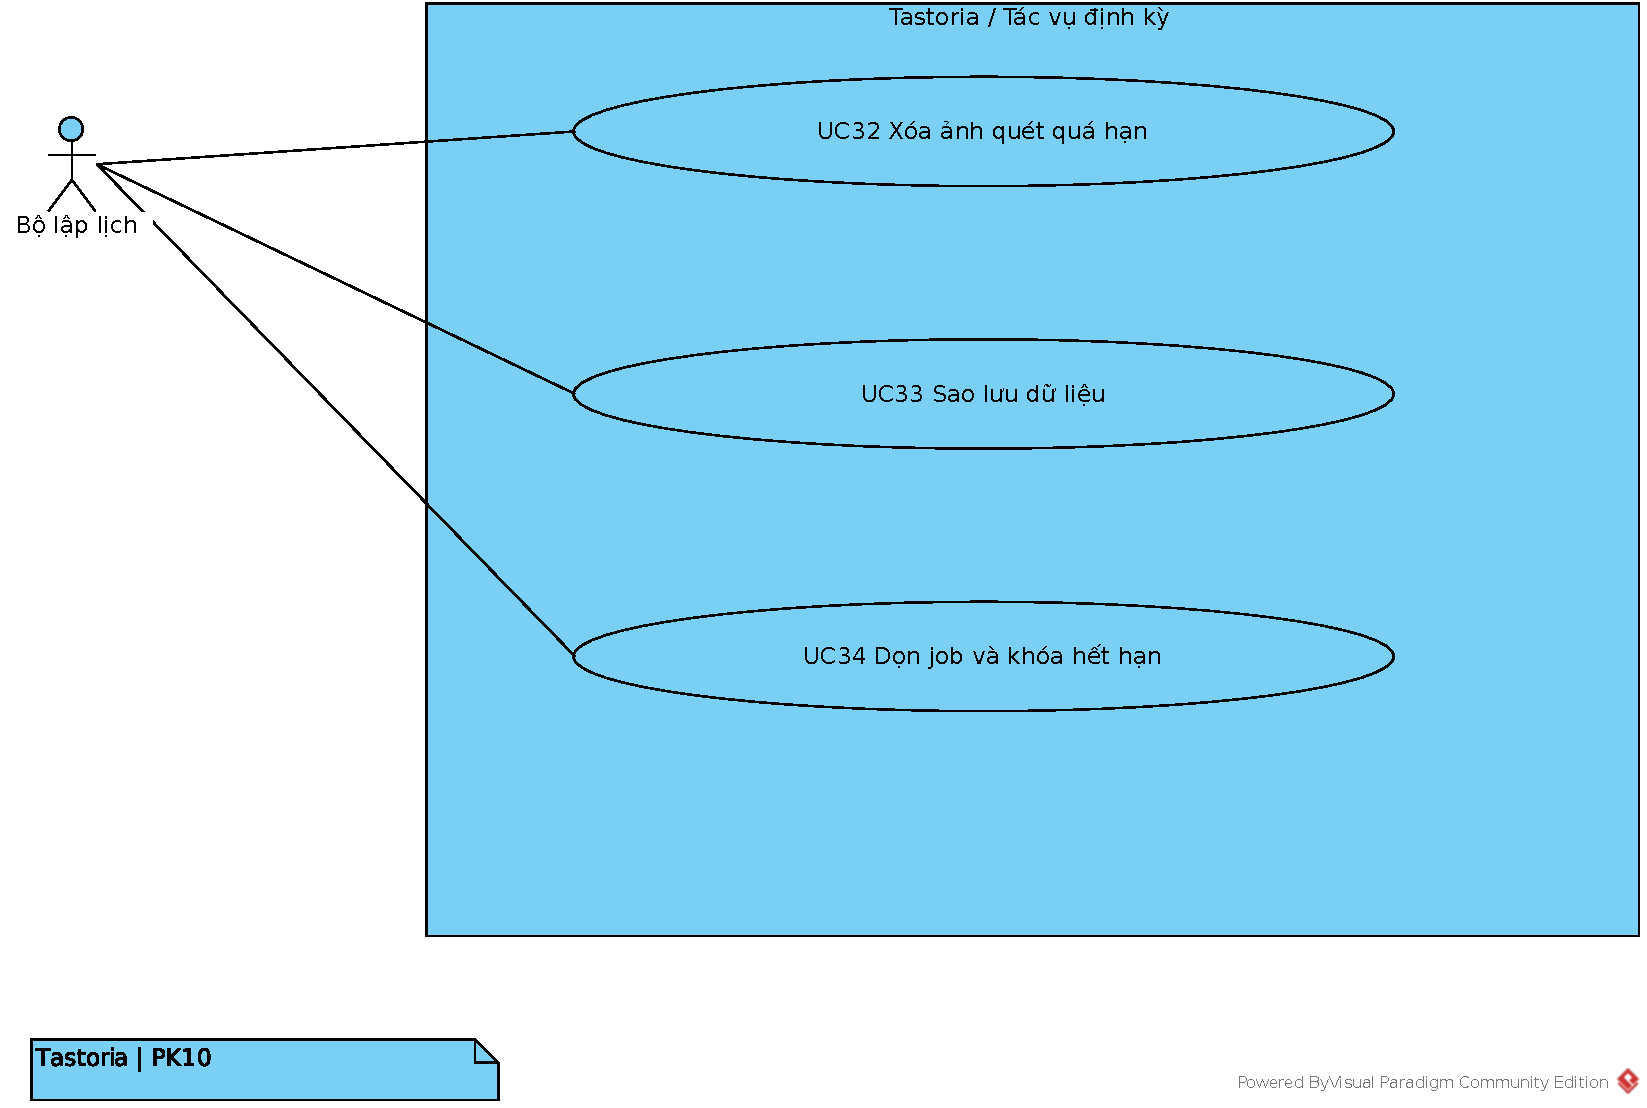
\includegraphics[width=0.96\linewidth,height=0.78\textwidth,keepaspectratio]{assets/PK10.pdf}
\caption{PK10 --- Phân rã use case}\label{fig:Phu-luc-A-Use-Cases:10}
\end{figure}
\end{landscape}\clearpage
\section{UC32 --- Xoá ảnh quét quá hạn}
\subsection{Mục tiêu trong ngữ cảnh}
Bộ lập lịch (A08) kích hoạt tác vụ xoá tệp ảnh quét gốc đã quá 30 ngày, trừ ảnh mà người dùng đã đồng ý góp và vẫn đang đồng ý. Tác vụ cũng xoá ảnh góp của người đã rút đồng ý {\small\texttt{photo\_\allowbreak{}\allowbreak{}contribution}}. Mục tiêu là hệ thống không giữ ảnh tủ lạnh lâu hơn quy định lưu giữ, và lần chạy nào cũng an toàn để chạy lại.

\subsection{Phạm vi và mức}
\begin{itemize}
\item Phạm vi: hệ thống Tastoria, container {\small\texttt{scheduler}} gọi {\small\texttt{python -\allowbreak{}m tastoria.\allowbreak{}jobs.\allowbreak{}purge\_\allowbreak{}\allowbreak{}images}}; module {\small\texttt{jobs}} gọi {\small\texttt{scan}} (xoá ảnh) và {\small\texttt{privacy}} (đồng ý, kiểm toán).
\item Mức: mục tiêu người dùng của tác nhân thời gian A08 (tác vụ nền; quy tắc gán mức ở SRS \S{}2.2).
\end{itemize}
\subsection{Tác nhân và bên liên quan (quyền lợi)}
{\footnotesize\setlength{\tabcolsep}{0pt}
\begin{longtable}{@{}L{7.850cm}@{\hspace{3mm}}L{7.850cm}@{}}
\caption{Tác nhân và bên liên quan (quyền lợi)}\\
\toprule
\textbf{Bên} & \textbf{Quyền lợi} \\
\midrule\endfirsthead
\multicolumn{2}{l}{\small\itshape Bảng \thetable{} (tiếp theo)}\\
\toprule
\textbf{Bên} & \textbf{Quyền lợi} \\
\midrule\endhead
\bottomrule\endfoot
A08 Bộ lập lịch & Kích hoạt đúng lịch; nhận mã thoát để ghi log. \\ \addlinespace[3pt]
A02 Người dùng & Ảnh tủ lạnh không bị giữ quá 30 ngày; rút đồng ý góp ảnh thì ảnh bị xoá \ensuremath{\leq} 24 giờ. \\ \addlinespace[3pt]
A06 Người vận hành mô hình & Ảnh góp hợp lệ không bị xoá nhầm. \\ \addlinespace[3pt]
Bên kiểm soát dữ liệu & Có bằng chứng thực hiện chính sách lưu giữ. \\ \addlinespace[3pt]
\end{longtable}}
\subsection{Tiền điều kiện}
\begin{enumerate}
\item Container {\small\texttt{scheduler}} chạy, crontab có lịch cho tác vụ.
\item Volume lưu tệp ({\small\texttt{tmp/\allowbreak{}\allowbreak{}}}, {\small\texttt{contrib/\allowbreak{}\allowbreak{}}}) gắn vào container chạy tác vụ.
\end{enumerate}
\subsection{Đảm bảo tối thiểu}
Không ảnh góp có đồng ý hiện hành nào bị xoá. Dòng {\small\texttt{scan\_\allowbreak{}\allowbreak{}images}} không bị xoá (giữ dữ liệu dẫn xuất); chỉ tệp bị xoá và {\small\texttt{purged\_\allowbreak{}\allowbreak{}at}} được đặt. Lỗi một tệp không chặn các tệp khác.

\subsection{Đảm bảo khi thành công}
Sau lần chạy, không còn {\small\texttt{scan\_\allowbreak{}\allowbreak{}images}} nào thoả: {\small\texttt{purged\_\allowbreak{}\allowbreak{}at}} NULL và (scan tạo trước now - 30 ngày và không phải ảnh góp có đồng ý hiện hành, hoặc là ảnh góp của người đã rút {\small\texttt{photo\_\allowbreak{}\allowbreak{}contribution}}).

\subsection{Kích hoạt}
Lịch cron của container {\small\texttt{scheduler}} (đề xuất hằng ngày; xem mục 16).

\subsection{Kịch bản chính}
\begin{enumerate}
\item A08 chạy {\small\texttt{python -\allowbreak{}m tastoria.\allowbreak{}jobs.\allowbreak{}purge\_\allowbreak{}\allowbreak{}images}}.
\item Module {\small\texttt{jobs}} lấy khoá tư vấn PostgreSQL (advisory lock) của tác vụ để không chạy chồng.
\item Module {\small\texttt{jobs}} gọi {\small\texttt{scan.\allowbreak{}list\_\allowbreak{}\allowbreak{}purgeable\_\allowbreak{}\allowbreak{}images(now)}}; module {\small\texttt{scan}} gọi {\small\texttt{privacy}} đọc {\small\texttt{v\_\allowbreak{}\allowbreak{}current\_\allowbreak{}\allowbreak{}consents}} (mục đích {\small\texttt{photo\_\allowbreak{}\allowbreak{}contribution}}) và trả danh sách {\small\texttt{scan\_\allowbreak{}\allowbreak{}images}} cần xoá: {\small\texttt{purged\_\allowbreak{}\allowbreak{}at}} NULL và [{\small\texttt{scans.\allowbreak{}created\_\allowbreak{}\allowbreak{}at}} < now - 30 ngày và không ({\small\texttt{contributed = true}} và chủ ảnh đang đồng ý)] hoặc [{\small\texttt{contributed = true}} và chủ ảnh không còn đồng ý].
\item Với từng ảnh (theo lô), module {\small\texttt{scan}} xoá tệp theo {\small\texttt{storage\_\allowbreak{}\allowbreak{}key}} khỏi volume, rồi đặt {\small\texttt{purged\_\allowbreak{}\allowbreak{}at = now}} cho dòng đó.
\item Module {\small\texttt{jobs}} gọi {\small\texttt{privacy.\allowbreak{}record\_\allowbreak{}\allowbreak{}audit()}} ghi một dòng tổng hợp (action {\small\texttt{retention.\allowbreak{}purge\_\allowbreak{}\allowbreak{}images}}, actor\_\allowbreak{}role {\small\texttt{scheduler}}, số ảnh xoá, số lỗi).
\item Module {\small\texttt{jobs}} nhả khoá, ghi log JSON và thoát mã 0.
\end{enumerate}
\subsection{Mở rộng}
\begin{itemize}
\item \textbf{2a. Lần chạy trước còn giữ khoá}: thoát mã 0 ngay, ghi log "đang chạy", không làm gì.
\item \textbf{3a. Không có ảnh cần xoá}: ghi {\small\texttt{audit\_\allowbreak{}\allowbreak{}log}} với 0 ảnh; thoát mã 0.
\item \textbf{4a. Tệp không còn trên đĩa} (đã bị xoá thủ công hoặc lần chạy trước dừng giữa xoá tệp và ghi DB): coi là đã xoá, vẫn đặt {\small\texttt{purged\_\allowbreak{}\allowbreak{}at}}, đếm vào cảnh báo.
\item \textbf{4b. Xoá tệp lỗi quyền hoặc lỗi I/\allowbreak{}O}: không đặt {\small\texttt{purged\_\allowbreak{}\allowbreak{}at}} cho ảnh đó, đếm lỗi, tiếp tục ảnh khác; thoát mã \ensuremath{\neq} 0 cuối lần chạy để hệ thống giám sát thấy.
\item \textbf{4c. Mất kết nối DB giữa chừng} (lỗi hệ thống): ảnh đã xoá tệp nhưng chưa đặt {\small\texttt{purged\_\allowbreak{}\allowbreak{}at}} sẽ được xử lý ở lần sau theo 4a; thoát mã \ensuremath{\neq} 0.
\item \textbf{4d. Chạy lại ngay sau một lần thành công} (lũy đẳng): danh sách rỗng (ảnh đã có {\small\texttt{purged\_\allowbreak{}\allowbreak{}at}}).
\item \textbf{*a. Quá thời gian}: tác vụ xử lý theo lô và commit từng lô; bị dừng giữa chừng thì lần sau làm tiếp.
\item \textbf{*b. Người dùng xoá tài khoản}: tệp ảnh được xoá theo UC07; UC32 không xử lý dòng đã bị xoá theo cascade.
\item Quan hệ include/\allowbreak{}extend: model.yaml không khai báo include/\allowbreak{}extend cho UC32.
\end{itemize}
\subsection{Ghi chú đối chiếu của báo cáo}
Giữ phạm vi yêu cầu của đặc tả nguồn; cần kiểm thử theo môi trường và phiên bản thực tế trước khi ghi kết quả nghiệm thu.

\textbf{Nguồn:} {\small\texttt{Tastoria/\allowbreak{}\allowbreak{}docs/\allowbreak{}\allowbreak{}sad/\allowbreak{}\allowbreak{}use-\allowbreak{}cases/\allowbreak{}\allowbreak{}UC32.\allowbreak{}md}}. Mã nghiệp vụ: BR-\allowbreak{}RETAIN-\allowbreak{}01, BR-\allowbreak{}CONSENT-\allowbreak{}01, BR-\allowbreak{}CONSENT-\allowbreak{}04.

\textbf{Dữ liệu liên quan:} {\small\texttt{scan\_\allowbreak{}\allowbreak{}images}}, {\small\texttt{scans}}, {\small\texttt{v\_\allowbreak{}\allowbreak{}current\_\allowbreak{}\allowbreak{}consents}}, {\small\texttt{audit\_\allowbreak{}\allowbreak{}log}}.

\textbf{Điểm giao tiếp:} {\small\texttt{CLI python -\allowbreak{}m tastoria.\allowbreak{}jobs.\allowbreak{}purge\_\allowbreak{}\allowbreak{}images}}.

\section{UC33 --- Sao lưu cơ sở dữ liệu}
\subsection{Mục tiêu trong ngữ cảnh}
Bộ lập lịch (A08) kích hoạt tác vụ sao lưu hằng ngày: chụp toàn bộ cơ sở dữ liệu bằng {\small\texttt{pg\_\allowbreak{}\allowbreak{}dump -\allowbreak{}Fc}}, mã hoá, đẩy ra Drive ngoài máy chủ bằng rclone, kiểm bản đã đẩy, rồi xoá các bản cũ theo chính sách giữ \ensuremath{\leq} 14 ngày (7 bản ngày + 1 bản tuần). Mục tiêu là khôi phục được với RPO \ensuremath{\leq} 24 giờ, RTO \ensuremath{\leq} 2 giờ, và dữ liệu đã xoá theo yêu cầu không sống trong bản sao lưu quá hạn xoá 20 ngày.

\subsection{Phạm vi và mức}
\begin{itemize}
\item Phạm vi: hệ thống Tastoria, container {\small\texttt{scheduler}} gọi {\small\texttt{python -\allowbreak{}m tastoria.\allowbreak{}jobs.\allowbreak{}backup}}; module {\small\texttt{jobs}} dùng {\small\texttt{core}} (cấu hình, lưu tệp) và gọi {\small\texttt{privacy}} ghi kiểm toán; đích ngoài là Drive qua rclone.
\item Mức: mục tiêu người dùng của tác nhân thời gian A08 (tác vụ nền; quy tắc gán mức ở SRS \S{}2.2).
\end{itemize}
\subsection{Tác nhân và bên liên quan (quyền lợi)}
{\footnotesize\setlength{\tabcolsep}{0pt}
\begin{longtable}{@{}L{7.850cm}@{\hspace{3mm}}L{7.850cm}@{}}
\caption{Tác nhân và bên liên quan (quyền lợi)}\\
\toprule
\textbf{Bên} & \textbf{Quyền lợi} \\
\midrule\endfirsthead
\multicolumn{2}{l}{\small\itshape Bảng \thetable{} (tiếp theo)}\\
\toprule
\textbf{Bên} & \textbf{Quyền lợi} \\
\midrule\endhead
\bottomrule\endfoot
A08 Bộ lập lịch & Kích hoạt đúng lịch, nhận mã thoát. \\ \addlinespace[3pt]
Nhóm vận hành & Khôi phục được khi mất máy chủ; biết ngay khi sao lưu hỏng. \\ \addlinespace[3pt]
A02 Người dùng & Dữ liệu (kể cả khảo sát, nhật ký) không mất; dữ liệu đã xoá không tồn tại lâu trong bản sao lưu. \\ \addlinespace[3pt]
Bên kiểm soát dữ liệu & Bản sao lưu được mã hoá; khoá không nằm cạnh bản dump. \\ \addlinespace[3pt]
\end{longtable}}
\subsection{Tiền điều kiện}
\begin{enumerate}
\item Container {\small\texttt{scheduler}} chạy; có quyền kết nối {\small\texttt{postgres}} bằng tài khoản chỉ đọc đủ để {\small\texttt{pg\_\allowbreak{}\allowbreak{}dump}}.
\item rclone đã cấu hình tới Drive; khoá mã hoá bản sao lưu cấu hình riêng, không nằm trên Drive.
\end{enumerate}
\subsection{Đảm bảo tối thiểu}
Bản sao lưu chưa kiểm xong không bao giờ thay thế hay gây xoá bản cũ. Không có bản dump chưa mã hoá nào rời máy chủ. Thất bại luôn cho mã thoát \ensuremath{\neq} 0 và log JSON.

\subsection{Đảm bảo khi thành công}
\begin{enumerate}
\item Trên Drive có một bản mới mã hoá, kiểm checksum khớp bản cục bộ.
\item Số bản trên Drive theo chính sách: tối đa 7 bản ngày gần nhất + 1 bản tuần, không bản nào cũ hơn 14 ngày.
\item Tệp tạm cục bộ đã xoá.
\end{enumerate}
\subsection{Kích hoạt}
Lịch cron hằng ngày của container {\small\texttt{scheduler}}.

\subsection{Kịch bản chính}
\begin{enumerate}
\item A08 chạy {\small\texttt{python -\allowbreak{}m tastoria.\allowbreak{}jobs.\allowbreak{}backup}}.
\item Module {\small\texttt{jobs}} lấy khoá tư vấn của tác vụ.
\item Module {\small\texttt{jobs}} chạy {\small\texttt{pg\_\allowbreak{}\allowbreak{}dump -\allowbreak{}Fc}} (một snapshot nhất quán) ra tệp tạm.
\item Module {\small\texttt{jobs}} kiểm bản dump đọc được ({\small\texttt{pg\_\allowbreak{}\allowbreak{}restore -\allowbreak{}-\allowbreak{}list}} thành công).
\item Module {\small\texttt{jobs}} mã hoá tệp bằng khoá sao lưu, tính sha256 bản mã hoá, xoá bản chưa mã hoá.
\item Module {\small\texttt{jobs}} đẩy bản mã hoá lên Drive bằng rclone với tên chứa ngày (và đánh dấu bản tuần vào ngày quy định).
\item Module {\small\texttt{jobs}} kiểm bản trên Drive (kích thước và checksum khớp).
\item Module {\small\texttt{jobs}} xoá trên Drive các bản ngoài chính sách: bản ngày ngoài 7 bản gần nhất, bản tuần cũ hơn bản tuần gần nhất, mọi bản cũ hơn 14 ngày.
\item Module {\small\texttt{jobs}} xoá tệp tạm, gọi {\small\texttt{privacy.\allowbreak{}record\_\allowbreak{}\allowbreak{}audit()}} (action {\small\texttt{backup.\allowbreak{}create}}, tên bản, sha256, số bản bị xoá), nhả khoá, thoát mã 0.
\end{enumerate}
\subsection{Mở rộng}
\begin{itemize}
\item \textbf{2a. Lần chạy trước còn giữ khoá}: thoát mã 0, không làm gì.
\item \textbf{3a. {\small\texttt{pg\_\allowbreak{}\allowbreak{}dump}} lỗi} (DB không sẵn sàng, hết dung lượng đĩa tạm): xoá tệp tạm, thoát mã \ensuremath{\neq} 0; không đụng tới bản cũ.
\item \textbf{4a. Bản dump không đọc được}: như 3a.
\item \textbf{5a. Khoá mã hoá chưa cấu hình}: thoát mã \ensuremath{\neq} 0, không đẩy bản chưa mã hoá.
\item \textbf{6a. Mất mạng hoặc Drive lỗi} (rclone thất bại): thử lại tối đa 3 lần với giãn cách tăng dần; vẫn lỗi thì thoát mã \ensuremath{\neq} 0, giữ bản mã hoá cục bộ để lần sau đẩy, không xoá bản cũ trên Drive.
\item \textbf{6b. Chạy lại trong cùng ngày} (lũy đẳng): bản cùng tên ngày bị thay bằng bản mới sau khi bản mới kiểm xong; số bản ngày không tăng.
\item \textbf{7a. Checksum trên Drive không khớp}: xoá bản lỗi trên Drive, thoát mã \ensuremath{\neq} 0, không chạy bước 8.
\item \textbf{8a. Xoá bản cũ thất bại}: thoát mã \ensuremath{\neq} 0 (bản mới vẫn hợp lệ); lần sau xoá tiếp.
\item \textbf{*a. Quá thời gian}: tác vụ có giới hạn tổng (đề xuất 30 phút); vượt thì dừng, dọn tệp tạm, thoát mã \ensuremath{\neq} 0.
\item \textbf{*b. Diễn tập khôi phục}: thực hiện bằng script khôi phục riêng (spec \S{}10), không thuộc luồng tự động này; kết quả diễn tập ghi vào báo cáo.
\item Quan hệ include/\allowbreak{}extend: model.yaml không khai báo include/\allowbreak{}extend cho UC33.
\end{itemize}
\subsection{Ghi chú đối chiếu của báo cáo}
Giữ phạm vi yêu cầu của đặc tả nguồn; cần kiểm thử theo môi trường và phiên bản thực tế trước khi ghi kết quả nghiệm thu.

\textbf{Nguồn:} {\small\texttt{Tastoria/\allowbreak{}\allowbreak{}docs/\allowbreak{}\allowbreak{}sad/\allowbreak{}\allowbreak{}use-\allowbreak{}cases/\allowbreak{}\allowbreak{}UC33.\allowbreak{}md}}. Mã nghiệp vụ: BR-\allowbreak{}RETAIN-\allowbreak{}01, BR-\allowbreak{}DSR-\allowbreak{}01.

\textbf{Dữ liệu liên quan:} {\small\texttt{idempotency\_\allowbreak{}\allowbreak{}keys}}, {\small\texttt{users}}, {\small\texttt{refresh\_\allowbreak{}\allowbreak{}tokens}}, {\small\texttt{password\_\allowbreak{}\allowbreak{}resets}}, {\small\texttt{consent\_\allowbreak{}\allowbreak{}purposes}}, {\small\texttt{policy\_\allowbreak{}\allowbreak{}versions}}, {\small\texttt{consent\_\allowbreak{}\allowbreak{}events}}, {\small\texttt{dsr\_\allowbreak{}\allowbreak{}requests}}, {\small\texttt{audit\_\allowbreak{}\allowbreak{}log}}, {\small\texttt{food\_\allowbreak{}\allowbreak{}groups}}, {\small\texttt{nutrient\_\allowbreak{}\allowbreak{}sources}}, {\small\texttt{food\_\allowbreak{}\allowbreak{}items}}, {\small\texttt{nutrients}}, {\small\texttt{food\_\allowbreak{}\allowbreak{}nutrients}}, {\small\texttt{allergen\_\allowbreak{}\allowbreak{}groups}}, {\small\texttt{diets}}, {\small\texttt{diet\_\allowbreak{}\allowbreak{}exclusions}}, {\small\texttt{ingredients}}, {\small\texttt{ingredient\_\allowbreak{}\allowbreak{}synonyms}}, {\small\texttt{ingredient\_\allowbreak{}\allowbreak{}allergens}}, {\small\texttt{ingredient\_\allowbreak{}\allowbreak{}units}}, {\small\texttt{qty\_\allowbreak{}\allowbreak{}levels}}, {\small\texttt{cooking\_\allowbreak{}\allowbreak{}methods}}, {\small\texttt{tags}}, {\small\texttt{recipes}}, {\small\texttt{recipe\_\allowbreak{}\allowbreak{}ingredients}}, {\small\texttt{recipe\_\allowbreak{}\allowbreak{}steps}}, {\small\texttt{recipe\_\allowbreak{}\allowbreak{}tags}}, {\small\texttt{recipe\_\allowbreak{}\allowbreak{}sources}}, {\small\texttt{recipe\_\allowbreak{}\allowbreak{}nutrition}}, {\small\texttt{vision\_\allowbreak{}\allowbreak{}classes}}, {\small\texttt{vision\_\allowbreak{}\allowbreak{}class\_\allowbreak{}\allowbreak{}ingredients}}, {\small\texttt{profiles}}, {\small\texttt{user\_\allowbreak{}\allowbreak{}allergens}}, {\small\texttt{user\_\allowbreak{}\allowbreak{}favorite\_\allowbreak{}\allowbreak{}recipes}}, {\small\texttt{user\_\allowbreak{}\allowbreak{}settings}}, {\small\texttt{pantry\_\allowbreak{}\allowbreak{}lots}}, {\small\texttt{pantry\_\allowbreak{}\allowbreak{}transactions}}, {\small\texttt{model\_\allowbreak{}\allowbreak{}versions}}, {\small\texttt{model\_\allowbreak{}\allowbreak{}version\_\allowbreak{}\allowbreak{}classes}}, {\small\texttt{model\_\allowbreak{}\allowbreak{}deployments}}, {\small\texttt{scans}}, {\small\texttt{scan\_\allowbreak{}\allowbreak{}images}}, {\small\texttt{scan\_\allowbreak{}\allowbreak{}items}}, {\small\texttt{detections}}, {\small\texttt{substitution\_\allowbreak{}\allowbreak{}pairs}}, {\small\texttt{ingredient\_\allowbreak{}\allowbreak{}embeddings}}, {\small\texttt{shopping\_\allowbreak{}\allowbreak{}items}}, {\small\texttt{meal\_\allowbreak{}\allowbreak{}plans}}, {\small\texttt{meal\_\allowbreak{}\allowbreak{}plan\_\allowbreak{}\allowbreak{}coeater\_\allowbreak{}\allowbreak{}allergens}}, {\small\texttt{meal\_\allowbreak{}\allowbreak{}plan\_\allowbreak{}\allowbreak{}pins}}, {\small\texttt{meal\_\allowbreak{}\allowbreak{}plan\_\allowbreak{}\allowbreak{}items}}, {\small\texttt{meal\_\allowbreak{}\allowbreak{}plan\_\allowbreak{}\allowbreak{}item\_\allowbreak{}\allowbreak{}substitutions}}, {\small\texttt{cook\_\allowbreak{}\allowbreak{}sessions}}, {\small\texttt{cook\_\allowbreak{}\allowbreak{}schedule\_\allowbreak{}\allowbreak{}entries}}, {\small\texttt{interactions}}, {\small\texttt{survey\_\allowbreak{}\allowbreak{}forms}}, {\small\texttt{survey\_\allowbreak{}\allowbreak{}form\_\allowbreak{}\allowbreak{}anchors}}, {\small\texttt{survey\_\allowbreak{}\allowbreak{}respondents}}, {\small\texttt{survey\_\allowbreak{}\allowbreak{}assignments}}, {\small\texttt{survey\_\allowbreak{}\allowbreak{}ratings}}, {\small\texttt{survey\_\allowbreak{}\allowbreak{}favorites}}, {\small\texttt{v\_\allowbreak{}\allowbreak{}current\_\allowbreak{}\allowbreak{}consents}}, {\small\texttt{v\_\allowbreak{}\allowbreak{}pantry\_\allowbreak{}\allowbreak{}lot\_\allowbreak{}\allowbreak{}balance}}, {\small\texttt{v\_\allowbreak{}\allowbreak{}journal\_\allowbreak{}\allowbreak{}days}}.

\textbf{Điểm giao tiếp:} {\small\texttt{CLI python -\allowbreak{}m tastoria.\allowbreak{}jobs.\allowbreak{}backup}}.

\section{UC34 --- Dọn job quét kẹt, token và khoá lũy đẳng hết hạn}
\subsection{Mục tiêu trong ngữ cảnh}
Bộ lập lịch (A08) kích hoạt tác vụ sweeper mỗi phút. Tác vụ (1) phát hiện lần quét kẹt ở {\small\texttt{queued}} hoặc {\small\texttt{processing}} do worker chết, hàng đợi mất job hay enqueue lỗi, rồi đưa lại vào hàng đợi hoặc đặt {\small\texttt{expired}} khi hết lượt hay quá tuổi; (2) xoá khoá lũy đẳng quá 48 giờ; (3) xoá refresh token và token đặt lại mật khẩu đã hết hạn. Mục tiêu là app không chờ vô hạn một lần quét, và các bảng tạm không phình ra.

\subsection{Phạm vi và mức}
\begin{itemize}
\item Phạm vi: hệ thống Tastoria, container {\small\texttt{scheduler}} gọi {\small\texttt{python -\allowbreak{}m tastoria.\allowbreak{}jobs.\allowbreak{}sweep}}; module {\small\texttt{jobs}} gọi {\small\texttt{scan}} (job kẹt), {\small\texttt{identity}} (token), {\small\texttt{core}} (khoá lũy đẳng).
\item Mức: mục tiêu người dùng của tác nhân thời gian A08 (tác vụ nền; quy tắc gán mức ở SRS \S{}2.2).
\end{itemize}
\subsection{Tác nhân và bên liên quan (quyền lợi)}
{\footnotesize\setlength{\tabcolsep}{0pt}
\begin{longtable}{@{}L{7.850cm}@{\hspace{3mm}}L{7.850cm}@{}}
\caption{Tác nhân và bên liên quan (quyền lợi)}\\
\toprule
\textbf{Bên} & \textbf{Quyền lợi} \\
\midrule\endfirsthead
\multicolumn{2}{l}{\small\itshape Bảng \thetable{} (tiếp theo)}\\
\toprule
\textbf{Bên} & \textbf{Quyền lợi} \\
\midrule\endhead
\bottomrule\endfoot
A08 Bộ lập lịch & Kích hoạt mỗi phút; tác vụ ngắn, không chạy chồng. \\ \addlinespace[3pt]
A02 Người dùng & Lần quét kẹt được chạy lại hoặc báo hết hạn rõ ("thử lại /\allowbreak{} nhập tay"), không quay vòng mãi. \\ \addlinespace[3pt]
Nhóm vận hành & Bảng {\small\texttt{idempotency\_\allowbreak{}\allowbreak{}keys}}, {\small\texttt{refresh\_\allowbreak{}\allowbreak{}tokens}}, {\small\texttt{password\_\allowbreak{}\allowbreak{}resets}} không phình; số lần quét lỗi đo được. \\ \addlinespace[3pt]
\end{longtable}}
\subsection{Tiền điều kiện}
\begin{enumerate}
\item Container {\small\texttt{scheduler}} chạy; {\small\texttt{valkey}} và {\small\texttt{postgres}} sẵn sàng.
\item Lần quét đã có các cột {\small\texttt{status}}, {\small\texttt{attempts}}, {\small\texttt{enqueued\_\allowbreak{}\allowbreak{}at}}, {\small\texttt{started\_\allowbreak{}\allowbreak{}at}}.
\end{enumerate}
\subsection{Đảm bảo tối thiểu}
Sweeper không bao giờ ghi vào kho ({\small\texttt{pantry\_\allowbreak{}\allowbreak{}lots}}, {\small\texttt{pantry\_\allowbreak{}\allowbreak{}transactions}}) và không chuyển lần quét sang {\small\texttt{done}} hay {\small\texttt{confirmed}}. Không xoá token còn hạn hay khoá lũy đẳng chưa đủ 48 giờ.

\subsection{Đảm bảo khi thành công}
\begin{enumerate}
\item Không còn lần quét nào ở {\small\texttt{queued}}/\allowbreak{}{\small\texttt{processing}} quá ngưỡng kẹt mà chưa được đưa lại hàng đợi hoặc đặt {\small\texttt{expired}}; không lần quét nào ở {\small\texttt{queued}}/\allowbreak{}{\small\texttt{processing}} quá 5 phút kể từ {\small\texttt{created\_\allowbreak{}\allowbreak{}at}}.
\item {\small\texttt{idempotency\_\allowbreak{}\allowbreak{}keys}} không còn dòng có {\small\texttt{created\_\allowbreak{}\allowbreak{}at}} < now - 48 giờ.
\item {\small\texttt{refresh\_\allowbreak{}\allowbreak{}tokens}} và {\small\texttt{password\_\allowbreak{}\allowbreak{}resets}} không còn dòng có {\small\texttt{expires\_\allowbreak{}\allowbreak{}at}} < now.
\end{enumerate}
\subsection{Kích hoạt}
Lịch cron mỗi phút của container {\small\texttt{scheduler}}.

\subsection{Kịch bản chính}
\begin{enumerate}
\item A08 chạy {\small\texttt{python -\allowbreak{}m tastoria.\allowbreak{}jobs.\allowbreak{}sweep}}.
\item Module {\small\texttt{jobs}} lấy khoá tư vấn của tác vụ.
\item Module {\small\texttt{jobs}} gọi {\small\texttt{scan.\allowbreak{}sweep\_\allowbreak{}\allowbreak{}stuck\_\allowbreak{}\allowbreak{}scans(now)}}; module {\small\texttt{scan}} chọn lần quét có {\small\texttt{status \ensuremath{\in} \{queued, processing\}}} và mốc gần nhất ({\small\texttt{started\_\allowbreak{}\allowbreak{}at}} nếu {\small\texttt{processing}}, {\small\texttt{enqueued\_\allowbreak{}\allowbreak{}at}} nếu {\small\texttt{queued}}) cũ hơn ngưỡng kẹt 60 giây.
\item Với lần quét có {\small\texttt{attempts}} < 3: module {\small\texttt{scan}} đặt {\small\texttt{status = queued}}, {\small\texttt{enqueued\_\allowbreak{}\allowbreak{}at = now}}, enqueue lại với {\small\texttt{job\_\allowbreak{}\allowbreak{}id = scan\_\allowbreak{}\allowbreak{}id}}; {\small\texttt{attempts}} không đổi (worker tăng {\small\texttt{attempts}} khi bắt đầu một lần chạy, sơ đồ ST01).
\item Với lần quét {\small\texttt{processing}} có {\small\texttt{attempts}} = 3 (đã chạy đủ 1 lần đầu + 2 lần thử lại), hoặc lần quét {\small\texttt{queued}}/\allowbreak{}{\small\texttt{processing}} có {\small\texttt{created\_\allowbreak{}\allowbreak{}at}} cũ hơn 5 phút: module {\small\texttt{scan}} đặt {\small\texttt{status = expired}}, {\small\texttt{error\_\allowbreak{}\allowbreak{}code = timeout}}, {\small\texttt{finished\_\allowbreak{}\allowbreak{}at = now}}. Lỗi suy luận (không phải quá giờ) do worker xử lý và kết thúc ở {\small\texttt{failed}} (UC12, FR-\allowbreak{}12-\allowbreak{}19), sweeper không đặt {\small\texttt{failed}}.
\item Module {\small\texttt{jobs}} gọi {\small\texttt{core}} xoá {\small\texttt{idempotency\_\allowbreak{}\allowbreak{}keys}} có {\small\texttt{created\_\allowbreak{}\allowbreak{}at}} < now - 48 giờ.
\item Module {\small\texttt{jobs}} gọi {\small\texttt{identity}} xoá {\small\texttt{refresh\_\allowbreak{}\allowbreak{}tokens}} có {\small\texttt{expires\_\allowbreak{}\allowbreak{}at}} < now và {\small\texttt{password\_\allowbreak{}\allowbreak{}resets}} có {\small\texttt{expires\_\allowbreak{}\allowbreak{}at}} < now.
\item Module {\small\texttt{jobs}} ghi log JSON (số lần quét đưa lại, số đặt {\small\texttt{expired}}, số dòng xoá mỗi bảng); khi có lần quét bị đặt {\small\texttt{expired}}, gọi {\small\texttt{privacy.\allowbreak{}record\_\allowbreak{}\allowbreak{}audit()}} ghi một dòng tổng hợp (action {\small\texttt{sweep.\allowbreak{}scans\_\allowbreak{}\allowbreak{}expired}}).
\item Module {\small\texttt{jobs}} nhả khoá, thoát mã 0.
\end{enumerate}
\subsection{Mở rộng}
\begin{itemize}
\item \textbf{2a. Lần chạy trước còn giữ khoá} (lần trước chạy quá 1 phút): thoát mã 0, không làm gì.
\item \textbf{3a. Không có gì để dọn}: thoát mã 0 với số đếm 0.
\item \textbf{4a. Enqueue lỗi} ({\small\texttt{valkey}} không sẵn sàng): không tăng {\small\texttt{attempts}}, giữ nguyên trạng thái; lần sau thử lại; thoát mã \ensuremath{\neq} 0.
\item \textbf{4b. Worker hoàn tất job đúng lúc sweeper đang xử lý} (tranh chấp): cập nhật trạng thái có điều kiện ({\small\texttt{WHERE status}} và mốc thời gian như đã đọc); worker thắng thì sweeper bỏ qua lần quét đó.
\item \textbf{4c. Job trùng trong hàng đợi}: {\small\texttt{job\_\allowbreak{}\allowbreak{}id = scan\_\allowbreak{}\allowbreak{}id}} nên hàng đợi không chạy hai job cho cùng lần quét; worker bỏ qua job của lần quét không còn ở {\small\texttt{queued}}.
\item \textbf{5a. App đang long-\allowbreak{}poll lần quét bị đặt {\small\texttt{expired}}}: {\small\texttt{GET /\allowbreak{}\allowbreak{}scans/\allowbreak{}\allowbreak{}\{id\}}} trả {\small\texttt{expired}} với {\small\texttt{error\_\allowbreak{}\allowbreak{}code = timeout}}; app hiện "thử lại /\allowbreak{} nhập tay" (thuộc UC12).
\item \textbf{6a. Lỗi DB khi xoá} (lỗi hệ thống): rollback phần đó, thoát mã \ensuremath{\neq} 0; lần sau làm lại (thao tác lũy đẳng).
\item \textbf{*a. Chạy lại ngay} (lũy đẳng): lần quét đã đưa lại có mốc mới nên không bị đưa lại lần nữa; dòng đã xoá không còn.
\item \textbf{*b. Quá thời gian}: mỗi phần xử lý theo lô có giới hạn; phần còn lại xử lý ở lần chạy sau.
\item Quan hệ include/\allowbreak{}extend: model.yaml không khai báo include/\allowbreak{}extend cho UC34.
\end{itemize}
\subsection{Ghi chú đối chiếu của báo cáo}
Giữ phạm vi yêu cầu của đặc tả nguồn; cần kiểm thử theo môi trường và phiên bản thực tế trước khi ghi kết quả nghiệm thu.

\textbf{Nguồn:} {\small\texttt{Tastoria/\allowbreak{}\allowbreak{}docs/\allowbreak{}\allowbreak{}sad/\allowbreak{}\allowbreak{}use-\allowbreak{}cases/\allowbreak{}\allowbreak{}UC34.\allowbreak{}md}}. Mã nghiệp vụ: BR-\allowbreak{}SCAN-\allowbreak{}02.

\textbf{Dữ liệu liên quan:} {\small\texttt{scans}}, {\small\texttt{idempotency\_\allowbreak{}\allowbreak{}keys}}, {\small\texttt{refresh\_\allowbreak{}\allowbreak{}tokens}}, {\small\texttt{password\_\allowbreak{}\allowbreak{}resets}}, {\small\texttt{audit\_\allowbreak{}\allowbreak{}log}}.

\textbf{Điểm giao tiếp:} {\small\texttt{CLI python -\allowbreak{}m tastoria.\allowbreak{}jobs.\allowbreak{}sweep}}.
